% ============================================================
%  يُترجَم بـ XeLaTeX  (في Overleaf: Menu → Compiler → XeLaTeX)
%  الخط: Amiri (متوفر في Overleaf، أو حمّله من github.com/aliftype/amiri)
% ============================================================
\documentclass[12pt,a4paper]{article}
\usepackage[a4paper,margin=1.7cm,top=2.3cm,bottom=2.9cm,headheight=15pt,footskip=1.5cm]{geometry}
\usepackage{amsmath,amssymb}
\usepackage{icomma}
\usepackage[english,bidi=default,layout=lists]{babel}
\babelprovide[import,main]{arabic}
\babelfont{rm}[Scale=1.08]{Amiri}
\babelfont{sf}[Scale=1.08]{Amiri}
\usepackage[most]{tcolorbox}
\usepackage{tikz}
\usetikzlibrary{arrows.meta,calc,shadings}
\usepackage{array}
\usepackage{colortbl}
\usepackage{fancyhdr}
\usepackage{titlesec}
\usepackage{enumitem}
\usepackage{collcell}
\usepackage{needspace}
\usepackage{etoolbox}
\newcolumntype{C}{>{\collectcell\ar}c<{\endcollectcell}}
\pretocmd{\section}{\Needspace{15\baselineskip}}{}{}
\pretocmd{\subsection}{\Needspace{11\baselineskip}}{}{}

\definecolor{cDef}{HTML}{1F4E9C}
\definecolor{cThm}{HTML}{B3261E}
\definecolor{cRem}{HTML}{2E7D32}
\definecolor{cEx}{HTML}{C76B00}
\definecolor{cMeth}{HTML}{6A1B9A}
\definecolor{cSol}{HTML}{00695C}
\definecolor{cSec}{HTML}{1F3A68}

\titleformat{\section}{\Large\bfseries\color{cSec}}{\thesection.}{0.6em}{}[{\color{cSec!60}\titlerule[1pt]}]
\titleformat{\subsection}{\large\bfseries\color{cThm!85!black}}{\thesubsection.}{0.5em}{}
\titlespacing*{\section}{0pt}{14pt}{8pt}
\titlespacing*{\subsection}{0pt}{10pt}{5pt}
\setlength{\parindent}{0pt}
\setlength{\parskip}{4pt}
\setlist{itemsep=2pt,topsep=3pt}

\newtcolorbox{arbox}[3][]{enhanced,
  colback=#2!5,colframe=#2!80!black,arc=2mm,boxrule=0.8pt,
  left=6pt,right=6pt,top=8pt,bottom=5pt,
  fonttitle=\bfseries,coltitle=white,
  title={\foreignlanguage{arabic}{#3}},
  attach boxed title to top right={xshift=-5mm,yshift=-3mm},
  boxed title style={colback=#2!80!black,arc=1.5mm,boxrule=0pt},
  before upper={\selectlanguage{arabic}},
  before skip=8pt,after skip=8pt,breakable,#1}
\newenvironment{BOX}[2]{\begin{otherlanguage}{english}\begin{arbox}{#1}{#2}}{\end{arbox}\end{otherlanguage}}
\newenvironment{tarif}[1][تعريف]{\begin{BOX}{cDef}{#1}}{\end{BOX}}
\newenvironment{khassia}[1][خاصية]{\begin{BOX}{cThm}{#1}}{\end{BOX}}
\newenvironment{molahada}[1][ملاحظة]{\begin{BOX}{cRem}{#1}}{\end{BOX}}
\newenvironment{mithal}[1][مثال]{\begin{BOX}{cEx}{#1}}{\end{BOX}}
\newenvironment{tariqa}[1][طريقة]{\begin{BOX}{cMeth}{#1}}{\end{BOX}}

\newcounter{exo}
\newenvironment{tamrin}[1]{\stepcounter{exo}\begin{BOX}{cSec}{التمرين \theexo: #1}}{\end{BOX}}
\newenvironment{hal}{\Needspace{12\baselineskip}\begin{otherlanguage}{english}\begin{arbox}[breakable]{cSol}{حل التمرين \theexo}}{\end{arbox}\end{otherlanguage}}

\newenvironment{LTR}{\begin{otherlanguage}{english}}{\end{otherlanguage}}
\newcommand{\ar}[1]{\foreignlanguage{arabic}{#1}}

\renewcommand{\dots}{\mathinner{\ldotp\ldotp\ldotp}}
\renewcommand{\ldots}{\mathinner{\ldotp\ldotp\ldotp}}
\renewcommand{\cdots}{\mathinner{\cdotp\cdotp\cdotp}}
\newcommand{\N}{\mathbb{N}}
\newcommand{\Z}{\mathbb{Z}}
\newcommand{\D}{\mathbb{D}}
\newcommand{\Q}{\mathbb{Q}}
\newcommand{\R}{\mathbb{R}}
\newcommand{\pgcd}{\operatorname{PGCD}}
\newcommand{\ppcm}{\operatorname{PPCM}}

% \NLseg{a}{b}{[}{]} ; \NLright{a}{[} ; \NLleft{b}{]}  (interval on a number line)
\newcommand{\NLseg}[4]{\begin{LTR}\begin{tikzpicture}[baseline=-0.6ex]
 \draw[-{Stealth[length=2mm]},gray!70](0,0)--(3.4,0);
 \draw[line width=2pt,cThm!80!black](0.7,0)--(2.7,0);
 \node[cThm!80!black,font=\LARGE] at (0.7,0){$#3$};
 \node[cThm!80!black,font=\LARGE] at (2.7,0){$#4$};
 \node[below=3pt,font=\footnotesize] at (0.7,0){$#1$};
 \node[below=3pt,font=\footnotesize] at (2.7,0){$#2$};
\end{tikzpicture}\end{LTR}}
\newcommand{\NLright}[2]{\begin{LTR}\begin{tikzpicture}[baseline=-0.6ex]
 \draw[-{Stealth[length=2mm]},gray!70](0,0)--(3.4,0);
 \draw[line width=2pt,cThm!80!black](1.3,0)--(3.3,0);
 \node[cThm!80!black,font=\LARGE] at (1.3,0){$#2$};
 \node[below=3pt,font=\footnotesize] at (1.3,0){$#1$};
\end{tikzpicture}\end{LTR}}
\newcommand{\NLleft}[2]{\begin{LTR}\begin{tikzpicture}[baseline=-0.6ex]
 \draw[-{Stealth[length=2mm]},gray!70](0,0)--(3.4,0);
 \draw[line width=2pt,cThm!80!black](0.05,0)--(2.1,0);
 \node[cThm!80!black,font=\LARGE] at (2.1,0){$#2$};
 \node[below=3pt,font=\footnotesize] at (2.1,0){$#1$};
\end{tikzpicture}\end{LTR}}

% ---------- social-media icons (pure TikZ) ----------
\definecolor{cFB}{HTML}{1877F2}
\definecolor{cTG}{HTML}{229ED9}
\definecolor{cIG1}{HTML}{FEDA75}
\definecolor{cIG2}{HTML}{D62976}
\definecolor{cIG3}{HTML}{4F5BD5}
\newcommand{\fbicon}{\begin{LTR}\begin{tikzpicture}[baseline=-0.75ex,x=1em,y=1em]
 \fill[cFB] (0,0) circle (0.55);
 \node[white,inner sep=0,font=\usefont{TU}{lmss}{bx}{n}\small] at (0.04,-0.02) {f};
\end{tikzpicture}\end{LTR}}
\newcommand{\igicon}{\begin{LTR}
\begin{tikzpicture}[baseline=-0.75ex,x=1em,y=1em]
 \shade[lower left=cIG1,lower right=cIG2,upper left=cIG2,upper right=cIG3,rounded corners=0.28em] (-0.55,-0.55) rectangle (0.55,0.55);
 \draw[white,line width=0.09em,rounded corners=0.18em] (-0.36,-0.36) rectangle (0.36,0.36);
 \draw[white,line width=0.09em] (0,0) circle (0.17);
 \fill[white] (0.22,0.22) circle (0.05);
\end{tikzpicture}\end{LTR}}
\newcommand{\tgicon}{\begin{LTR}
\begin{tikzpicture}[baseline=-0.75ex,x=1em,y=1em]
 \fill[cTG] (0,0) circle (0.55);
 \fill[white] (-0.33,0.0) -- (0.32,0.27) -- (0.2,-0.3) -- (0.0,-0.15) -- (-0.08,-0.28) -- (-0.08,-0.08) -- cycle;
 \fill[cTG!70!black] (-0.08,-0.08) -- (0.25,0.2) -- (0.0,-0.15) -- (-0.08,-0.28) -- cycle;
\end{tikzpicture}\end{LTR}}
% page number: black box, white two-digit number, at the right of the social row
\newcommand{\PageBox}{\begin{LTR}\tikz[baseline=(p.base)]\node[fill=black,text=white,inner sep=2.5pt,minimum width=1.6em,minimum height=1.3em,font=\usefont{TU}{lmss}{bx}{n}\small](p){\ifnum\value{page}<10 0\fi\arabic{page}};\end{LTR}}
% visual left-to-right order: Telegram | Instagram | Facebook | page box
\newcommand{\SocialRow}{\begin{otherlanguage}{english}%
 \ar{\textbf{الأستاذ سوايسية هشام للرياضيات}}\ \tgicon\hfill
 \textbf{prof\_hicham\_math}\ \igicon\hfill
 \ar{\textbf{الأستاذ سوايسية هشام للرياضيات}}\ \fbicon\hspace{2.2em}\PageBox\end{otherlanguage}}

\pagestyle{fancy}
\fancyhf{}
\renewcommand{\headrulewidth}{0.6pt}
\renewcommand{\footrulewidth}{0.4pt}
% \SetHeader{right head: document title}{left head: level -- stream}
\newcommand{\SetHeader}[2]{%
 \fancyhead[C]{\parbox{\textwidth}{\ar{#1\hfill #2}}}%
 \fancyfoot[C]{\parbox{\textwidth}{\small\SocialRow}}}
\usepackage{tkz-tab}
\usepackage{multicol}
% variation / sign table (LTR)
\newenvironment{TAB}{\par\begin{center}\begin{LTR}\begin{tikzpicture}[scale=0.95,every node/.style={font=\small}]}{\end{tikzpicture}\end{LTR}\end{center}}
% grid + axes, clipped: \begin{GR}{xmin}{xmax}{ymin}{ymax}{unit cm}
\newenvironment{GR}[5]{\par\begin{center}\begin{LTR}\begin{tikzpicture}[x=#5cm,y=#5cm,font=\footnotesize]
 \draw[gray!25,very thin] (#1,#3) grid (#2,#4);
 \draw[-{Stealth[length=2mm]}] (#1,0)--(#2+0.3,0) node[below left]{$x$};
 \draw[-{Stealth[length=2mm]}] (0,#3)--(0,#4+0.3) node[below left]{$y$};
 \node[below left] at (0,0){$O$};
 \begin{scope}\clip (#1,#3) rectangle (#2,#4);}
{\end{scope}\end{tikzpicture}\end{LTR}\end{center}}
\newcommand{\Ticks}[2]{\foreach \t in {#1} \node[below,font=\scriptsize] at (\t,0){$\t$}; \foreach \t in {#2} \node[left,font=\scriptsize] at (0,\t){$\t$};}
\newcommand{\bx}[1]{\ensuremath{\colorbox{cDef!12}{$\displaystyle #1$}}}
\newcommand{\TwoCol}[4]{\par\begin{LTR}\noindent\begin{minipage}[t]{#1\textwidth}\selectlanguage{arabic}#2\end{minipage}\hfill\begin{minipage}[t]{#3\textwidth}\selectlanguage{arabic}#4\end{minipage}\end{LTR}\par}
\newcommand{\RL}[4]{\TwoCol{#3}{#4}{#1}{#2}}  % \RL{w1}{right content}{w2}{left content}
\newcommand{\ok}{$\textcolor{cRem}{\checkmark}$}
\newcommand{\limn}{\displaystyle\lim_{n\to+\infty}}
% sub-questions, each on its own line
\newenvironment{sq}{\begin{itemize}[leftmargin=2.4em,itemsep=3pt]}{\end{itemize}}
\newcommand{\qa}{\item[(أ)]}\newcommand{\qb}{\item[(ب)]}\newcommand{\qc}{\item[(جـ)]}\newcommand{\qd}{\item[(د)]}\newcommand{\qe}{\item[(هـ)]}
\newcommand{\pa}{\par\smallskip\textbf{(أ)} }\newcommand{\pb}{\par\smallskip\textbf{(ب)} }\newcommand{\pc}{\par\smallskip\textbf{(جـ)} }\newcommand{\pd}{\par\smallskip\textbf{(د)} }\newcommand{\pe}{\par\smallskip\textbf{(هـ)} }
\newcommand{\QQ}[1]{\par\smallskip\textbf{#1.} }
\newenvironment{tmr}{\stepcounter{exo}\begin{BOX}{cSec}{تمرين \theexo}}{\end{BOX}}
\newcommand{\ABC}[3]{\\[2pt]\begin{tabular}{p{0.28\textwidth}p{0.28\textwidth}p{0.28\textwidth}}(جـ) \ #3 & (ب) \ #2 & (أ) \ #1\end{tabular}}
\pretocmd{\section}{\Needspace{24\baselineskip}}{}{}
\newtcbox{\bxtbox}{on line,colback=cDef!12,colframe=cDef!12,boxrule=0pt,arc=1pt,boxsep=0pt,left=2pt,right=2pt,top=1pt,bottom=1pt}
\newcommand{\bxt}[1]{\foreignlanguage{english}{\bxtbox{\ar{#1}}}}
\SetHeader{\small\bfseries\color{cSec}تمارين تجريبية: الاحتمالات}{\small\color{cSec}السنة الثالثة ثانوي -- الشعب العلمية}
\begin{document}
\begin{LTR}
\begin{tcolorbox}[enhanced,colback=cSec,colframe=cSec,arc=3mm,halign=center,boxrule=0pt,top=12pt,bottom=12pt,before upper={\selectlanguage{arabic}}]
{\color{white}\fontsize{26}{32}\selectfont\bfseries تمارين تجريبية في الاحتمالات}\\[8pt]
{\color{white}\large تمارين متدرجة -- بدون حلول (للتدرّب)}\\[5pt]
{\color{white}\large السنة الثالثة ثانوي -- الشعب العلمية}
\end{tcolorbox}
\end{LTR}
% ================= تمارين تدريبية: الاحتمالات =================
\section{العدّ}

\begin{tamrin}{القوائم والترتيبات: الرمز السري}
رمز سري لهاتف يتكون من 4 أرقام مأخوذة من بين الأرقام $0,1,2,\ldots,9$ (مثلًا: $0725$ أو $3311$).
\QQ{1} ما عدد الرموز السرية الممكنة؟
\QQ{2} ما عدد الرموز المكونة من 4 أرقام مختلفة مثنى مثنى؟
\QQ{3} ما عدد الرموز المكونة من 4 أرقام مختلفة مثنى مثنى ولا تبدأ بالرقم $0$؟
\QQ{4} ما عدد الرموز التي تحتوي على الرقم $0$ مرة واحدة على الأقل؟
\end{tamrin}

\begin{tamrin}{التوفيقات: تشكيل لجنة}
قسم به 20 تلميذًا: 12 بنتًا و8 أولاد. نريد تشكيل لجنة من 3 تلاميذ.
\QQ{1} ما عدد اللجان الممكنة؟
\QQ{2} ما عدد اللجان المكونة من بنتين وولد واحد بالضبط؟
\QQ{3} ما عدد اللجان التي تضم ولدًا واحدًا على الأقل؟
\QQ{4} علي تلميذ من هذا القسم. ما عدد اللجان التي يكون علي عضوًا فيها؟
\QQ{5} نريد الآن اختيار رئيس ونائب رئيس وكاتب (3 مهام مختلفة لثلاثة تلاميذ مختلفين). ما عدد الإمكانيات؟
\end{tamrin}

\begin{tamrin}{التبديلات: ترتيب كتب على رف}
نرتب على رف 5 كتب رياضيات مختلفة و3 كتب فيزياء مختلفة.
\QQ{1} ما عدد الترتيبات الممكنة؟
\QQ{2} ما عدد الترتيبات التي تكون فيها كتب الرياضيات متجاورة؟
\QQ{3} ما عدد الترتيبات التي تكون فيها كتب كل مادة متجاورة؟
\QQ{4} ما عدد الترتيبات التي لا يتجاور فيها أي كتابي فيزياء؟
\end{tamrin}

\section{السحب في آن واحد وعلى التوالي}

\begin{tamrin}{سحب في آن واحد}
يحتوي كيس على 9 كريات متماثلة لا نفرق بينها باللمس: 4 حمراء، 3 خضراء وكريتان بيضاوان. نسحب عشوائيًا وفي آن واحد 3 كريات.
\QQ{1} ما عدد الحالات الممكنة؟
\QQ{2} احسب احتمال كل حدث من الأحداث التالية:
\begin{sq}
\qa $A$: «الكريات الثلاث من نفس اللون».
\qb $B$: «الكريات الثلاث مختلفة الألوان مثنى مثنى».
\qc $C$: «سحب كرية بيضاء على الأقل».
\qd $D$: «سحب كريتين حمراوين بالضبط».
\end{sq}
\end{tamrin}

\begin{tamrin}{سحب على التوالي بإرجاع وبدون إرجاع}
صندوق به 6 كريات متماثلة: ثلاث تحمل الرقم $1$، اثنتان تحملان الرقم $2$ وواحدة تحمل الرقم $0$.
\QQ{1} نسحب عشوائيًا كريتين على التوالي دون إرجاع.
\begin{sq}
\qa ما عدد الحالات الممكنة؟
\qb احسب احتمال الحدث $A$: «مجموع الرقمين يساوي 2».
\qc احسب احتمال الحدث $B$: «جداء الرقمين معدوم».
\qd احسب احتمال الحدث $C$: «الكرية الثانية تحمل الرقم 2».
\end{sq}
\QQ{2} نعيد التجربة لكن بالسحب على التوالي مع الإرجاع. احسب في هذه الحالة $P(A)$ و$P(B)$.
\end{tamrin}

\begin{tamrin}{مقارنة أنواع السحب الثلاثة}
كيس به 5 كريات متماثلة: 3 بيضاء و2 سوداء. نسحب كريتين وفق كل نمط من الأنماط التالية:
(I) في آن واحد، (II) على التوالي دون إرجاع، (III) على التوالي مع إرجاع.
\QQ{1} في كل نمط، احسب عدد الحالات الممكنة.
\QQ{2} في كل نمط، احسب احتمال الحدث $E$: «الكريتان من نفس اللون» واحتمال الحدث $F$: «الكريتان مختلفتا اللون».
\QQ{3} في النمطين (II) و(III)، احسب احتمال الحدث $G$: «الأولى بيضاء والثانية سوداء».
\QQ{4} ماذا تلاحظ؟
\end{tamrin}

\section{قانون الاحتمال والمتغير العشوائي}

\begin{tamrin}{لعبة بنرد}
نرمي نردًا متوازنًا وجوهه مرقمة من 1 إلى 6. إذا ظهر الرقم 6 يربح اللاعب 10 نقاط، وإذا ظهر 4 أو 5 يربح نقطتين، وفي باقي الحالات يخسر 3 نقاط. ليكن $X$ المتغير العشوائي الذي يرفق بكل رمية ربح اللاعب (الخسارة ربح سالب).
\QQ{1} عيّن قيم $X$ ثم عرّف قانون احتماله.
\QQ{2} احسب الأمل الرياضياتي $E(X)$. هل اللعبة في صالح اللاعب؟
\QQ{3} احسب التباين $V(X)$ والانحراف المعياري $\sigma(X)$.
\QQ{4} احسب $P(X>0)$.
\end{tamrin}

\begin{tamrin}{عدد الكريات السوداء المسحوبة}
يحتوي صندوق على 4 كريات بيضاء و3 كريات سوداء، متماثلة لا نفرق بينها باللمس. نسحب عشوائيًا وفي آن واحد 3 كريات. ليكن $X$ المتغير العشوائي الذي يرفق بكل سحب عدد الكريات السوداء المسحوبة.
\QQ{1} عيّن قيم $X$ ثم عرّف قانون احتماله.
\QQ{2} احسب $E(X)$ و$V(X)$ و$\sigma(X)$.
\QQ{3} احسب $P(X\geqslant2)$ ثم $P(X^2-X=0)$.
\end{tamrin}

\begin{tamrin}{مجموع رقمين وتحويل تآلفي}
صندوق به 6 كريات متماثلة: كريتان تحملان الرقم $-1$، ثلاث كريات تحمل الرقم $0$ وكرية واحدة تحمل الرقم $2$. نسحب عشوائيًا وفي آن واحد كريتين. ليكن $X$ المتغير العشوائي الذي يرفق بكل سحب مجموع الرقمين المسجلين.
\QQ{1} بيّن أن قيم $X$ هي: $-2$، $-1$، $0$، $1$، $2$.
\QQ{2} عرّف قانون احتمال $X$.
\QQ{3} احسب $E(X)$ و$V(X)$ و$\sigma(X)$.
\QQ{4} احسب $P(|X|\leqslant1)$.
\QQ{5} نعتبر المتغير العشوائي $Y=2X+1$. استنتج $E(Y)$ و$V(Y)$.
\end{tamrin}

\section{الاحتمال الشرطي وشجرة الاحتمالات -- رياضيات وعلوم تجريبية}

\begin{tamrin}{جدول بمدخلين والاحتمال الشرطي}
في ثانوية بها 200 تلميذ في السنة الثالثة: 120 بنتًا و80 ولدًا. من بين البنات 90 يدرسن في شعبة علمية، ومن بين الأولاد 50 يدرسون في شعبة علمية. نختار تلميذًا عشوائيًا. نسمي $F$: «التلميذ بنت» و$S$: «التلميذ في شعبة علمية».
\QQ{1} أكمل الجدول بمدخلين التالي:
\begin{center}
\begin{tabular}{|C|C|C|C|}\hline
\rowcolor{cSec!12} المجموع & $\overline{S}$ & $S$ & \\\hline
$120$ & $\ldots$ & $90$ & $F$\\\hline
$\ldots$ & $\ldots$ & $50$ & $\overline{F}$\\\hline
$200$ & $\ldots$ & $\ldots$ & المجموع\\\hline
\end{tabular}
\end{center}
\QQ{2} احسب $P(F)$، $P(S)$ و$P(F\cap S)$.
\QQ{3} احسب $P_F(S)$ ثم $P_S(F)$، وفسّر كل نتيجة.
\end{tamrin}

\begin{tamrin}{ثلاث آلات: الاحتمالات الكلية والسؤال العكسي}
مصنع ينتج قطعًا بثلاث آلات: الآلة $M_1$ تنتج $50\%$ من الإنتاج، و$M_2$ تنتج $30\%$، و$M_3$ تنتج الباقي. نسبة القطع المعيبة هي $2\%$ لإنتاج $M_1$، و$3\%$ لإنتاج $M_2$، و$5\%$ لإنتاج $M_3$. نختار قطعة عشوائيًا من الإنتاج الكلي. نسمي $D$: «القطعة معيبة» و$M_i$: «القطعة من إنتاج الآلة $M_i$».
\QQ{1} مثّل الوضعية بشجرة احتمالات.
\QQ{2} احسب $P(M_1\cap D)$.
\QQ{3} بيّن أن $P(D)=0.029$.
\QQ{4} القطعة المختارة معيبة. ما احتمال أن تكون من إنتاج الآلة $M_3$؟
\end{tamrin}

\begin{tamrin}{صندوقان ونرد}
لدينا صندوقان: $U_1$ به 3 كريات بيضاء و2 حمراء، و$U_2$ به كرية بيضاء واحدة و3 حمراء. نرمي نردًا متوازنًا: إذا ظهر 1 أو 2 نسحب كرية من $U_1$، وإلا نسحب كرية من $U_2$. نسمي $U_1$: «السحب من الصندوق $U_1$» و$B$: «الكرية المسحوبة بيضاء».
\QQ{1} أنشئ شجرة الاحتمالات المناسبة.
\QQ{2} بيّن أن $P(B)=\dfrac{11}{30}$.
\QQ{3} علمًا أن الكرية المسحوبة بيضاء، ما احتمال أنها سُحبت من $U_1$؟
\QQ{4} علمًا أن الكرية المسحوبة حمراء، ما احتمال أنها سُحبت من $U_1$؟
\end{tamrin}

\begin{tamrin}{سحب مع إضافة كرية من نفس اللون}
يحتوي صندوق على 3 كريات حمراء وكريتين خضراوين. نسحب كرية، نسجل لونها ثم نعيدها إلى الصندوق ونضيف معها كرية أخرى من نفس لونها، ثم نسحب كرية ثانية. نسمي $R_1$: «الكرية الأولى حمراء» و$R_2$: «الكرية الثانية حمراء».
\QQ{1} احسب $P_{R_1}(R_2)$ و$P_{\overline{R_1}}(R_2)$، ثم أنشئ شجرة الاحتمالات.
\QQ{2} احسب $P(R_2)$. قارنه بـ $P(R_1)$.
\QQ{3} علمًا أن الكرية الثانية حمراء، ما احتمال أن تكون الأولى حمراء أيضًا؟
\QQ{4} احسب احتمال الحدث $E$: «الكريتان من نفس اللون».
\end{tamrin}

\section{الاستقلالية -- رياضيات وعلوم تجريبية}

\begin{tamrin}{حدثان مستقلان}
\QQ{1} $A$ و$B$ حدثان مستقلان من فضاء احتمالي حيث $P(A)=0.4$ و$P(B)=0.5$. احسب:
\begin{sq}
\qa $P(A\cap B)$ و$P(A\cup B)$.
\qb $P(\overline{A}\cap\overline{B})$ ثم تحقق أنه يساوي $P(\overline{A})\times P(\overline{B})$.
\qc $P(A\cap\overline{B})$.
\end{sq}
\QQ{2} نرمي نردًا متوازنًا مرة واحدة. نعتبر الأحداث: $A$: «ظهور رقم زوجي»، $B$: «ظهور رقم أصغر من أو يساوي 2»، $C$: «ظهور رقم أكبر من أو يساوي 4».
\begin{sq}
\qa هل الحدثان $A$ و$B$ مستقلان؟
\qb هل الحدثان $A$ و$C$ مستقلان؟
\end{sq}
\end{tamrin}

\begin{tamrin}{دارة بثلاث مركبات مستقلة}
جهاز يحتوي على ثلاث مركبات $C_1$، $C_2$، $C_3$ تعمل باستقلالية عن بعضها. احتمال أن تعمل كل منها خلال سنة هو على الترتيب: $0{,}9$ ، $0{,}8$ ، $0{,}7$.
\QQ{1} احسب احتمال أن تعمل المركبات الثلاث (تركيب على التسلسل).
\QQ{2} احسب احتمال أن تتعطل مركبة واحدة على الأقل.
\QQ{3} احسب احتمال أن تعمل مركبة واحدة على الأقل (تركيب على التفرع).
\QQ{4} احسب احتمال أن تعمل مركبة واحدة فقط.
\QQ{5} في الجهاز، $C_1$ مركبة على التسلسل مع المجموعة ($C_2$ و$C_3$ على التفرع) كما في الشكل. يعمل الجهاز إذا مر التيار من $E$ إلى $S$. احسب احتمال أن يعمل الجهاز.
\begin{center}\begin{LTR}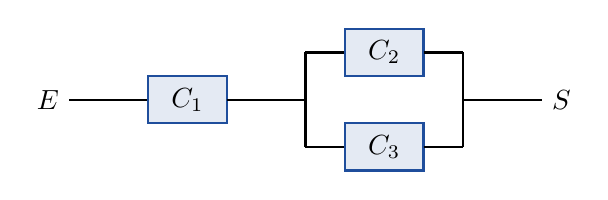
\begin{tikzpicture}[thick,b/.style={draw=cDef,fill=cDef!12,minimum width=10mm,minimum height=6mm}]
\node[left] at (0,0){$E$};
\draw (0,0)--(1,0); \node[b] (c1) at (1.5,0){$C_1$}; \draw (2,0)--(3,0);
\draw (3,0.6)--(3,-0.6); \draw (3,0.6)--(3.5,0.6); \draw (3,-0.6)--(3.5,-0.6);
\node[b] at (4,0.6){$C_2$}; \node[b] at (4,-0.6){$C_3$};
\draw (4.5,0.6)--(5,0.6); \draw (4.5,-0.6)--(5,-0.6); \draw (5,0.6)--(5,-0.6); \draw (5,0)--(6,0);
\node[right] at (6,0){$S$};
\end{tikzpicture}\end{LTR}\end{center}
\end{tamrin}

\section{اختيار من متعدد وصحيح أم خطأ}

\begin{tamrin}{اختيار من متعدد}
اختر الإجابة الصحيحة الوحيدة في كل حالة مع التعليل.

\textbf{1.} عدد طرق جلوس 4 أشخاص على 4 كراسي مصفوفة هو:
\ABC{$16$}{$24$}{$4$}\par\medskip

\textbf{2.} العدد $C_7^3$ يساوي:
\ABC{$35$}{$210$}{$21$}\par\medskip

\textbf{3.} نسحب في آن واحد كريتين من كيس به 6 كريات. عدد الحالات الممكنة هو:
\ABC{$30$}{$36$}{$15$}\par\medskip

\textbf{4.} (رياضيات وعلوم تجريبية) $A$ و$B$ مستقلان، $P(A)=0.3$ و$P(B)=0.6$. إذن $P(A\cup B)$ يساوي:
\ABC{$0{,}9$}{$0{,}72$}{$0{,}18$}\par\medskip

\textbf{5.} متغير عشوائي $X$ يأخذ القيم $-1$، $0$، $2$ باحتمالات $0{,}3$، $0{,}5$، $0{,}2$ على الترتيب. $E(X)$ يساوي:
\ABC{$0{,}1$}{$0{,}7$}{$0$}\par\medskip

\textbf{6.} (رياضيات وعلوم تجريبية) $P(A)=0.5$، $P_A(B)=0.4$ و$P(\overline{A}\cap B)=0.1$. إذن $P(B)$ يساوي:
\ABC{$0{,}2$}{$0{,}5$}{$0{,}3$}
\end{tamrin}

\begin{tamrin}{صحيح أم خطأ}
أجب بـ «صحيح» أو «خطأ» مع التعليل ($n$ و$p$ عددان طبيعيان، $0\leqslant p\leqslant n$).

\textbf{1.} $A_n^p=p!\times C_n^p$.\par
\textbf{2.} (رياضيات وعلوم تجريبية) إذا كان $A$ و$B$ حدثين غير متلائمين واحتمال كل منهما غير معدوم، فإنهما مستقلان.\par
\textbf{3.} $C_n^p=C_n^{n-p}$.\par
\textbf{4.} إذا كان $V(X)=4$ فإن $V(3X+1)=37$.\par
\textbf{5.} عدد الكلمات المكونة من 3 حروف (لها معنى أو لا) من الحروف $a$، $b$، $c$، $d$ مع إمكانية التكرار هو $64$.\par
\textbf{6.} نرمي قطعة نقدية متوازنة 3 مرات. احتمال الحصول على الوجه مرتين بالضبط هو $\dfrac14$.
\end{tamrin}

\section{النمذجة والمحاكاة}

\begin{tamrin}{نمذجة اختيار المندوبين بسحب كريات}
قسم به $30$ تلميذًا منهم $18$ بنتًا. نختار عشوائيًا وفي آن واحد $3$ تلاميذ لتمثيل القسم. ليكن $X$ عدد البنات المختارات.
\QQ{1} اقترح تجربة مرجعية (سحب من كيس) تنمذج هذه الوضعية، واحسب $\operatorname{card}\Omega$.
\QQ{2} عرّف قانون احتمال $X$.
\QQ{3} احسب $E(X)$ وفسّر النتيجة.
\end{tamrin}

\begin{tamrin}{هل حجر النرد الرباعي متوازن؟ -- شعبة علوم تجريبية}
حجر نرد رباعي الأوجه مرقم من $1$ إلى $4$. رميناه $100$ مرة فحصلنا على:
\begin{center}
\begin{tabular}{|C|c|c|c|c|C|}\hline
\rowcolor{cSec!12} الوجه & $1$ & $2$ & $3$ & $4$ & المجموع\\\hline
العدد $n_i$ & $14$ & $36$ & $20$ & $30$ & $100$\\\hline
\end{tabular}
\end{center}
\QQ{1} احسب التواترات $f_i$، ثم المؤشر $d^2=\displaystyle\sum_{i=1}^{4}\Big(f_i-\frac14\Big)^2$.
\QQ{2} حاكينا بالمجدول $1000$ سلسلة من $100$ رمية لنرد رباعي متوازن، وحسبنا $d^2$ لكل سلسلة، فكان العشير التاسع لهذه القيم $D_9\approx0{,}0158$. هل المعطيات ملائمة لنموذج نرد متوازن بخطر $10\%$؟
\QQ{3} أعاد تلميذ التجربة ($100$ رمية) بحجر آخر فحصل على الأعداد $18;30;22;30$. ما قرارك؟
\end{tamrin}

\section{تمارين شعبة رياضيات}

\begin{tamrin}{لعبة يتعلق أملها بوسيط -- شعبة رياضيات}
$n$ عدد طبيعي غير معدوم. صندوق به 3 كريات سوداء و$n$ كرية بيضاء، متماثلة لا نفرق بينها باللمس. يسحب لاعب عشوائيًا وفي آن واحد كريتين. إذا كانتا مختلفتي اللون يربح نقطة واحدة، وإذا كانتا من نفس اللون يخسر نقطة واحدة. ليكن $X$ المتغير العشوائي الذي يرفق بكل سحب ربح اللاعب الجبري.
\QQ{1} بيّن أن احتمال سحب كريتين مختلفتي اللون هو $\dfrac{6n}{(n+3)(n+2)}$.
\QQ{2} عرّف قانون احتمال $X$ ثم بيّن أن $E(X)=\dfrac{-(n-1)(n-6)}{(n+3)(n+2)}$.
\QQ{3} عيّن قيم $n$ التي تكون من أجلها اللعبة عادلة، ثم قيم $n$ التي تكون من أجلها اللعبة في صالح اللاعب.
\QQ{4} عيّن قيم $n$ التي يكون من أجلها $E(X)$ أكبر ما يمكن.
\QQ{5} نضع $n=3$. احسب $V(X)$ و$\sigma(X)$.
\end{tamrin}

\begin{tamrin}{مطابقات التوفيقات واختيار جزء عشوائي -- شعبة رياضيات}
$n$ عدد طبيعي غير معدوم و$E$ مجموعة بها $n$ عنصرًا.
\QQ{1} بيّن أنه من أجل كل عدد طبيعي $p$ حيث $1\leqslant p\leqslant n$: \quad $p\,C_n^p=n\,C_{n-1}^{p-1}$.\par
أعط تفسيرًا تعداديًا لهذه المساواة (لجنة من $p$ أشخاص لها رئيس).
\QQ{2} باستعمال دستور ثنائي الحد، بيّن أن $\displaystyle\sum_{k=0}^{n}C_n^k=2^n$، ثم استنتج أن $\displaystyle\sum_{k=1}^{n}k\,C_n^k=n\,2^{n-1}$.
\QQ{3} بيّن أن $\displaystyle\sum_{k=0}^{n}(-1)^kC_n^k=0$، واستنتج أن عدد الأجزاء من $E$ التي عدد عناصرها زوجي هو $2^{n-1}$.
\QQ{4} نختار عشوائيًا جزءًا من $E$ (كل الأجزاء لها نفس الاحتمال). ليكن $X$ عدد عناصر الجزء المختار.
\begin{sq}
\qa بيّن أن $P(X=k)=\dfrac{C_n^k}{2^n}$ من أجل $0\leqslant k\leqslant n$.
\qb استنتج أن $E(X)=\dfrac n2$، واحتمال أن يكون عدد عناصر الجزء زوجيًا.
\qc في حالة $n=4$، عرّف قانون احتمال $X$ وتحقق من قيمة $E(X)$.
\end{sq}
\end{tamrin}

\end{document}
